%=======================02-713 LaTeX template, following the 15-210 template==================
%
% You don't need to use LaTeX or this template, but you must turn your homework in as
% a typeset PDF somehow.
%
% How to use:
%    1. Update your information in section "A" below
%    2. Write your answers in section "B" below. Precede answers for all 
%       parts of a question with the command "\question{n}{desc}" where n is
%       the question number and "desc" is a short, one-line description of 
%       the problem. There is no need to restate the problem.
%    3. If a question has multiple parts, precede the answer to part x with the
%       command "\part{x}".
%    4. If a problem asks you to design an algorithm, use the commands
%       \algorithm, \correctness, \runtime to precede your discussion of the 
%       description of the algorithm, its correctness, and its running time, respectively.
%    5. You can include graphics by using the command \includegraphics{FILENAME}
%
\documentclass[11pt]{article}
\usepackage{amsmath,amssymb,amsthm}
\usepackage{mathtools}
\usepackage{tikz}
\usetikzlibrary{arrows,positioning, calc}
\tikzstyle{vertex}=[draw,fill=black!15,circle,minimum size=20pt,inner sep=0pt]
\usepackage{graphicx}
\usepackage[margin=1in]{geometry}
\usepackage{fancyhdr}
\usepackage{mathtools}
\usepackage{placeins}
\usepackage{listings}
\usepackage{color}

\definecolor{dkgreen}{rgb}{0,0.6,0}
\definecolor{gray}{rgb}{0.5,0.5,0.5}
\definecolor{mauve}{rgb}{0.58,0,0.82}

\lstset{frame=none,
  language=Python,
  aboveskip=3mm,
  belowskip=3mm,
  showstringspaces=false,
  columns=flexible,
  basicstyle={\small\ttfamily},
  numbers=none,
  numberstyle=\tiny\color{gray},
  keywordstyle=\color{blue},
  commentstyle=\color{dkgreen},
  stringstyle=\color{mauve},
  breaklines=true,
  breakatwhitespace=true,
  tabsize=3
}

\setlength{\parindent}{0pt}
\setlength{\parskip}{5pt plus 1pt}
\setlength{\headheight}{13.6pt}
\newcommand\question[2]{\vspace{.25in}\hrule\textbf{#1 #2}\vspace{.5em}\hrule\vspace{.10in}}
\renewcommand\part[1]{\vspace{.10in}\textbf{(#1)}}
\newcommand\algorithm{\vspace{.10in}\textbf{Algorithm: }}
\newcommand\correctness{\vspace{.10in}\textbf{Correctness: }}
\newcommand\runtime{\vspace{.10in}\textbf{Running time: }}
\pagestyle{fancyplain}
\lhead{\textbf{\NAME}}
\chead{\textbf{HW\HWNUM}}
\rhead{\today}
\begin{document}\raggedright
%Section A==============Change the values below to match your information==================
\newcommand\NAME{Sean Connor}  % your name
\newcommand\HWNUM{10}              % the homework number
%Section B==============Put your answers to the questions below here=======================

\question{Q1}{}
If no record with the key is present, then for an unordered table sequential search will always evaluate the entire table, or n entries. If the table is ordered, then the best case would be a single evaluation, the worst case would be $n$ evaluations, and the average case would be $\frac{n}{2}$ evaluations. Here is example pseudocode to demonstrate this:

\begin{lstlisting}
# Pseudocode for sequential search of unordered list
for Item in Table:
	if Item.key == key:   # key found, return key
		return Item
return null              # entire table evaluated, key not found, return null


# Pseudocode for sequential search of ordered list
for Item in Table:
	if Item.key == key:   # key found, return key
		return Item
	elif Item.key > key: # search moved past possible, key not in table, return null
		return null
return null               # entire table evaluated, key not found, return null
	
\end{lstlisting}

\question{Q2}{}
If one record with the key is present and only one record is sought, then the efficiency will not depend at all on whether the table is ordered or unordered. In both cases, the best case would be a single evaluation, the worst case would be $n$ evaluations, and the average case would be $\frac{n}{2}$ evaluations. 

\question{Q3}{}
If more than one record with the key is present and it is desired to find only the first, then the efficiency will not depend at all on whether the table is ordered or unordered. In both cases, the best case would be a single evaluation, the worst case would be $n-m$ evaluations, and the average case would be $\frac{n}{2}$ evaluations. 

\question{Q4}{}
If more than one record with the key is present and it is desired to find them all, for an unordered list sequential search will perform a $m$ comparisons in the best case, $n-m$ comparisons in the worst case, and $\frac{n}{2}$ comparisons in the average case. 

If the list is sorted, then any record with the same key as the first found will be located immediately after the first record. Thus, the performance is the same; that is, the best case will require a single comparison, the worst case will require $n-m$ comparisons, and the average case will require $\frac{n}{2}$ comparisons.

\question{Q5}{}
This question is perhaps best answered with a demonstration. In this example we search for the two largest numbers in the set [1, 2, 3, 4, 100, 110, 120, 130].
\begin{figure}[h!]
\centering
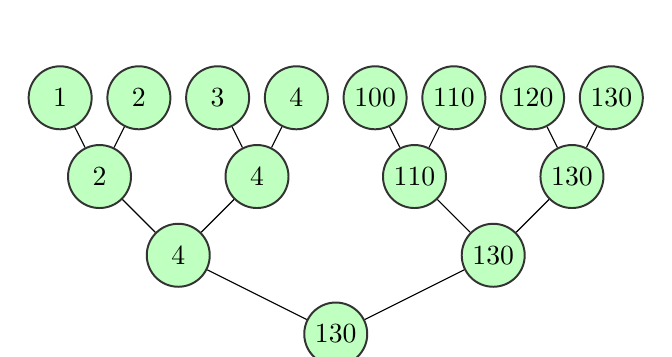
\begin{tikzpicture}
[level distance=10mm,
every node/.style={draw=black!80,fill=green!25,circle,inner sep=0pt,line width=.25mm,minimum size=.8cm},
level 1/.style={sibling distance=40mm},
level 2/.style={sibling distance=20mm},
level 3/.style={sibling distance=10mm}]
\node  {130} [grow=up]
child {node {130}
child {node {130}
child {node {130}}
child {node {120}}
}
child {node {110}
child {node {110}}
child {node {100}}
}
}
child {node {4}
child {node {4}
child {node {4}}
child {node {3}}
}
child {node {2}
child {node {2}}
child {node {1}}
}
};
\end{tikzpicture}
\caption{This is part one of the search, where each set of leaf nodes is compared to each other and the greater of the two ``moves on''. There are a total of $n-1$ comparisons made.}
\end{figure}

\begin{figure}[h!]
\centering
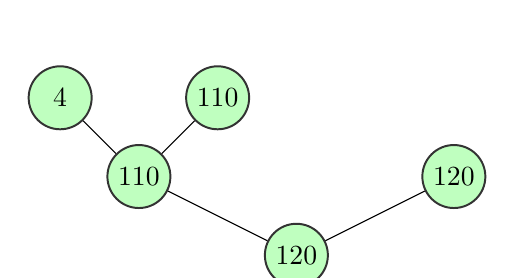
\begin{tikzpicture}
[level distance=10mm,
every node/.style={draw=black!80,fill=green!25,circle,inner sep=0pt,line width=.25mm,minimum size=.8cm},
level 1/.style={sibling distance=40mm},
level 2/.style={sibling distance=20mm},
level 3/.style={sibling distance=10mm}]
\node  {120} [grow=up]
child {node {120}
}
child {node {110}
child {node {110}}
child {node {4}}
};
\newline
\end{tikzpicture}
\caption{This is part two of the search, where the ``loser'' values at each level are compared in order to find the second largest value. There are a total of $(log_2 n) - 1$ comparisons made. The total number of comparisons then is $n + (log_2 n) - 2$.}
\end{figure}

\pagebreak
\question{Q6}{}
This question builds off of the previous question. We saw in Question 5 that it takes $n-1$ comparisons to find the largest value in a set. To find the smallest we do almost the same thing, except there are two differences. First, the initial (level 0) comparisons have already been made. Second, we are looking for the smaller value, and not the larger value in this case.

Thus, we can simply take the smaller values from the level 0 comparisons and perform an additional $\frac{n}{2} - 1$ comparisons to find the smallest value. The total number of comparisons then is $\frac{3n}{2}-2$.

\begin{figure}[h!]
\centering
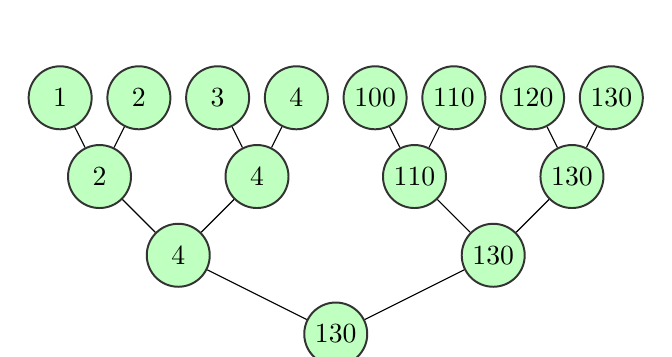
\begin{tikzpicture}
[level distance=10mm,
every node/.style={draw=black!80,fill=green!25,circle,inner sep=0pt,line width=.25mm,minimum size=.8cm},
level 1/.style={sibling distance=40mm},
level 2/.style={sibling distance=20mm},
level 3/.style={sibling distance=10mm}]
\node  {130} [grow=up]
child {node {130}
child {node {130}
child {node {130}}
child {node {120}}
}
child {node {110}
child {node {110}}
child {node {100}}
}
}
child {node {4}
child {node {4}
child {node {4}}
child {node {3}}
}
child {node {2}
child {node {2}}
child {node {1}}
}
};
\end{tikzpicture}
\caption{This is part one of the search, where we find the greastest value in the set. There are a total of $n-1$ comparisons made.}
\end{figure}

\begin{figure}[h!]
\centering
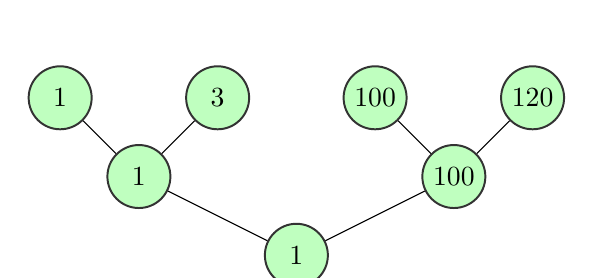
\begin{tikzpicture}
[level distance=10mm,
every node/.style={draw=black!80,fill=green!25,circle,inner sep=0pt,line width=.25mm,minimum size=.8cm},
level 1/.style={sibling distance=40mm},
level 2/.style={sibling distance=20mm},
level 3/.style={sibling distance=10mm}]
\node  {1} [grow=up]
child {node {100}
child {node {120}}
child {node {100}}
}
child {node {1}
child {node {3}}
child {node {1}}
};
\end{tikzpicture}
\caption{This is part two of the search, where we find the smallest value in the set. The initial level 0 comparisons were already made when finding the greatest value, so we only need to do $\frac{n}{2}-1$ comparisons. The total number of comparisons then is $\frac{3n}{2} - 2$.}
\end{figure}

\question{Q7}{}
For a list with $n$ records, there are $n!$ ways of ordering. However, achieving a straight-line (maximum height) binary tree is only possible in two cases - perfect ascending or perfect descending order. Thus, the probability of a max height binary tree is $\frac{2}{n!}$. 

Consider the example using a set of numbers [1, 2, 3, 4, 5, 6, 7]. There are two possible ways to achieve a maximum height - inserting in order [1, 2, 3, 4, 5, 6, 7] or inserting in order [7, 6, 5, 4, 3, 2, 1]. However, if we look at the case of the perfectly balanced tree, we see there at least 56 ways of ordering.

\pagebreak
\begin{figure}[h!]
\centering
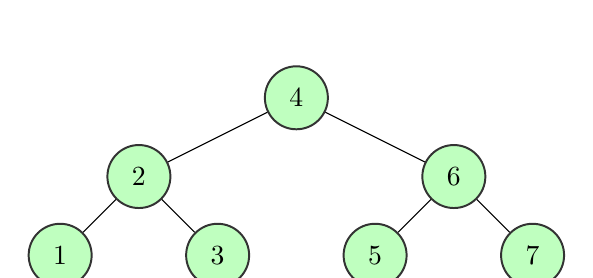
\begin{tikzpicture}
[level distance=10mm,
every node/.style={draw=black!80,fill=green!25,circle,inner sep=0pt,line width=.25mm,minimum size=.8cm},
level 1/.style={sibling distance=40mm},
level 2/.style={sibling distance=20mm},
level 3/.style={sibling distance=10mm}]
\node  {4} [grow=down]
child {node {2}
child {node {1}}
child {node {3}}
}
child {node {6}
child {node {5}}
child {node {7}}
};
\end{tikzpicture}
\end{figure}

For example, the following orders all produce the same tree: \newline
[4, 2, 6, 1, 3, 5, 7] \newline
[4, 2, 6, 1, 3, 7, 5] \newline
[4, 2, 6, 1, 5, 3, 7] \newline
[4, 2, 6, 1, 5, 7, 3] \newline
[4, 2, 6, 1, 7, 3, 5] \newline
[4, 2, 6, 1, 7, 5, 3] \newline
. \newline
. \newline
. \newline

From this, it is clear that balanced trees are more probable than straight-line trees.

\question{Q8}{}
\begin{lstlisting}
# Pseudocode for delete(key1,key2) method
delete(key1,key2)
	key = key1
	while key <= key2:
		delete(key)
		key++

# Pseudocode for delete(key) method
delete(key)
	# find node
	for node in tree:
		if node.key == key:
			current = node
	
	# remove leaf node
	if current.left == null AND current.right == null:
		if current.parent.left == current:
			current.parent.left == null
		elif current.parent.right == current: 
			current.parent.right == null
		else:
			tree.root = null
	
	# remove node with only left child
	if current.left != null AND current.right == null:
		if current.parent.left == current:
			current.parent.left == current.left
		elif current.parent.right == current: 
			current.parent.right == current.left
		else:
			tree.root = null
	
	# remove node with only right child
	if current.left == null AND current.right != null:
		if current.parent.left == current:
			current.parent.left == current.right
		elif current.parent.right == current: 
			current.parent.right == current.right
		else:
			tree.root = null
	
	# remove node with two children
	if current.left != null AND current.right != null:
		successor = current.right
		while successor.left != null:
			successor = successor.left
		current = successor
		remove(successor.key)

\end{lstlisting}

\question{Q9 }{}
This is a somewhat difficult question as there are several possible cases that can be encountered when deleting from a B-tree that need to be addressed. We must traverse from the root node to the node with desired key so that we can merge nodes that have less than the minimum number of keys.

\begin{lstlisting}
# Pseudocode for removal of a record from a B-Tree
delete(tree, key)
	current = tree.root
	while current != null:
		# preemptive merge
		if current.numberKeys == 1 AND current != tree.root
			Merge(current)
	
		if current.hasKey(key):
			# leaf node
			if current.isLeaf():
				RemoveKey(key)
				return true
				
			# internal node
			else
				copy(successor,key)
				delete(successor)
				return true
			
		current = Next(current, key)
	
	return false
\end{lstlisting}

\pagebreak
\question{Q10}{}
The first item inserted to the table will have no chance of collision, as all spaces are free. After this however, the chance of collision is represented by the number of items in the table divided by the table size. So for the n\textsuperscript{th} key, the collision probability will be $(n-1)/tablesize$. If we sum the collision probabilities of each successive addition, we find the following:

\begin{align*}
\sum_{0}^{n-1} \frac{n}{tablesize} &= \frac{1}{tablesize} +  \frac{2}{tablesize} + ... + \frac{n-1}{tablesize} \\
&= \frac{1}{tablesize}\left(\frac{n(n-1)}{2}\right) \\
&= \frac{n}{tablesize}\left(\frac{n-1}{2}\right) \\
&= (n-1)\frac{lf}{2}
\end{align*}

\question{Q11}{}
The maximum number of comparisons done is equal to $1+tablesize$. If we divide this by the number of open spots plus one, we will have the average number of comparisons needed to insert a new element. That is, if no spots are open, then the maximum number of comparisons occurs and if all spots are open then only a single comparison occurs. The number of open spots is given by $n_{open} = tablesize - n$. Thus, the final equation becomes:
\begin{align*}
\frac{tablesize+1}{tablesize-n+1}
\end{align*}
Linear probing does not satisfy this condition because it simply inserts into the next available space if a bucket is occupied. It would need random selection to satisfy the above.

\end{document}









